\subsection{Bài tập về thiết bị khuấy trộn liên tục}
\subsubsection{Mô hình về hai bình chứa chất lỏng nối tiếp nhau}
    \begin{figure}[htp]
        \begin{center}
            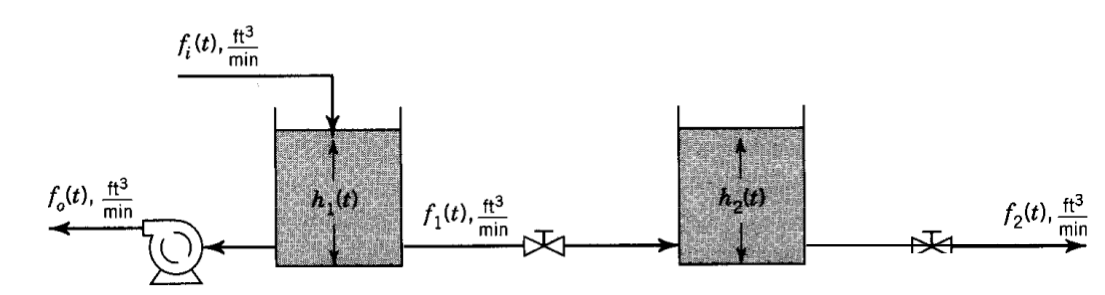
\includegraphics[scale=0.4]{section/mohinhhoalythuyet/images/binhchuachatlong-2binh}
        \end{center}
        \caption{Mô hình về hai bình chứa chất lỏng nối tiếp nhau} \label{Fig:binhchuachatlong-2binh}
    \end{figure}

\subparagraph{Các đại lượng trên mô hình}
    \begin{itemize}
		\item $f_i, f_o, f_1, f_2$: Lưu lượng lưu lượng dòng nguyên liệu $\pfm{ft^3/min}$.
		\item $h_1, h_2$: Mức chất lỏng trong bình $\pfm{m}$.
        \item $A_1, A_2$: Tiết diện của bình chứa $\pfm{m^2}$.
        \item Giả sử đặc tính qua van tuyến tính và lưu lượng qua van được xác định bằng công thức sau: $F = C_v \sqrt{\dfrac{\Delta P}{G_f}}$ với $C_v$ là hệ số van $\pfm{ft^3/s.kPa^{\sfrac{1}{2}}}$, $\Delta P$ là độ chêch lệnh áp suất qua van $\pfm{kPa}$ và $G_f$ là trọng lượng riêng của chất lỏng.
	\end{itemize}

\subparagraph{Mô tả quá trình} Duy trì mức chất lỏng trong mỗi bình ở mức $h_1$ và $h_2$.

\subsubsection{Xác định các biến quá trình}
    \begin{center}
        \begin{tabular}{l|l}
            Biến vào: $f_i, f_o, f_1, f_2$ & Biến điều khiển: $f_1, f_2$ \\ \hline
            Biến ra: $h_1, h_2$ & Biến cần điều khiển: $h_1, h_2$\\ \hline
            & Biến nhiễu: $f_1, f_o$
        \end{tabular}
    \end{center}

\subsubsection{Xây dựng phương trình toán học}
    \begin{itemize}
        \item Xác định lưu lượng dòng chảy qua mỗi van:
            \begin{itemize}
                \item Van 1, ta có: $\Delta P = \pfm{\rho g h_1 + P_a} - \pfm{\rho g h_2 + P_a} = \rho g h_1 - \rho g h_2 = \rho g \pfm{h_1 - h_2}$, nên: $f_1 = C_{v_1} \sqrt{\dfrac{\Delta P}{G_f}} = C_{v_2} \sqrt{\dfrac{\rho g \pfm{h_1 - h_2}}{G_f}} = C_{v_1}^{*}\sqrt{h_1 - h_2}$ với $C_{v_1}^{*} = C_{v_1} \sqrt{\dfrac{\rho g}{G_f}}$.
                \item Van 2, ta có: $\Delta P = \pfm{\rho g h_2 + P_a} - P_a = \rho g h_2$, nên: $f_2 = C_{v_2} \sqrt{\dfrac{\Delta P}{G_f}} = C_{v_2} \sqrt{\dfrac{\rho g h_2}{G_f}} = C_{v_2}^{*}\sqrt{h_2}$ với $C_{v_2}^{*} = C_{v_2} \sqrt{\dfrac{\rho g}{G_f}}$.
            \end{itemize}
        \item Công thức tính thể tích $V = Ah$ với $A$ là tiết diện của bình chứa.
        \item Áp dụng phương trình cân bằng vật chất cho bình chứa 1:
            \begin{align*}
                \dfrac{dV_1}{dt} = f_i - \pfm{f_o + f_1} \Longleftrightarrow \dfrac{d\pfm{A_1 h_1}}{dt} = f_i - f_o - f_1 \Longleftrightarrow \dfrac{dh_1}{dt} = \dfrac{1}{A_1} \pfm{f_i - f_o - f_1}
            \end{align*}
            \item Áp dụng phương trình cân bằng vật chất cho bình chứa 1:
                \begin{align*}
                    \dfrac{dV_2}{dt} = f_1 - f_2 \Longleftrightarrow \dfrac{d\pfm{A_2 h_2}}{dt} = f_1 - f_2 \Longleftrightarrow \dfrac{dh_2}{dt} = \dfrac{1}{A_2} \pfm{f_1 - f_2}
                \end{align*}
        \item Kết luận, mô hình toán của hệ thống là:
            \begin{align*}
                \left\{\begin{array}{l}
                    \dfrac{dh_1}{dt} = \dfrac{1}{A_1} \pfm{f_i - f_o - f_1}\\ [.5cm]
                    \dfrac{dh_2}{dt} = \dfrac{1}{A_2} \pfm{f_1 - f_2}
                \end{array}\right.
            \end{align*}
        \item Thay $f_1 = C_{v_1}^{*}\sqrt{h_1 - h_2}$ và $f_2 = C_{v_2}^{*}\sqrt{h_2}$ (với $C_{v_1}^{*} = C_{v_1} \sqrt{\dfrac{\rho g}{G_f}}$ và $C_{v_2}^{*} = C_{v_2} \sqrt{\dfrac{\rho g}{G_f}}$), ta có:
            \begin{align*}
                \left\{\begin{array}{l}
                    \dfrac{dh_1}{dt} = \dfrac{1}{A_1} \pfm{f_i - f_o - C_{v_1}^{*}\sqrt{h_1 - h_2}}\\[.5cm]
                    \dfrac{dh_2}{dt} = \dfrac{1}{A_2} \pfm{C_{v_1}^{*}\sqrt{h_1 - h_2} - C_{v_2}^{*}\sqrt{h_2}} \\ [.5cm]
                    C_{v_1}^{*} = C_{v_1} \sqrt{\dfrac{\rho g}{G_f}}; \quad C_{v_2}^{*} = C_{v_2} \sqrt{\dfrac{\rho g}{G_f}}
                \end{array}\right.
            \end{align*}
    \end{itemize}

\subsubsection{Tuyến tính hóa phương trình quanh điểm làm việc cân bằng}
    \begin{itemize}
        \item Đặt: $h_1 = \overline{h}_1 + \Delta h_1$; $h_2 = \overline{h}_2 + \Delta h_2$; $f_i = \overline{f}_i + \Delta f_i$; $f_o = \overline{f}_o + \Delta f_o$.
        \item Tại điểm làm việc cân bằng $(\overline{h}_1, \overline{h}_2, \overline{f}_i, \overline{f}_o)$, ta có:
            \begin{align*}
                \left\{\begin{array}{l}
                    \dfrac{dh_1}{dt} = \dfrac{1}{A_1} \pfm{\overline{f}_i - \overline{f}_o - C_{v_1}^{*}\sqrt{\overline{h}_1 - \overline{h}_2}} = 0\\[.5cm]
                    \dfrac{dh_2}{dt} = \dfrac{1}{A_2} \pfm{C_{v_1}^{*}\sqrt{\overline{h}_1 - \overline{h}_2} - C_{v_2}^{*}\sqrt{\overline{h}_2}} = 0\\ [.5cm]
                \end{array}\right.
                \Longleftrightarrow
                \left\{\begin{array}{l}
                     \overline{f}_i - \overline{f}_o - C_{v_1}^{*}\sqrt{\overline{h}_1 - \overline{h}_2} = 0 \\ [.5cm]
                    C_{v_1}^{*}\sqrt{\overline{h}_1 - \overline{h}_2} - C_{v_2}^{*}\sqrt{\overline{h}_2} = 0
                \end{array}\right.
            \end{align*}
        \item Khai triển Taylor cho $f(f_i, f_o, h_1, h_2) = \dfrac{dh_1}{dt} = \dfrac{1}{A_1} \pfm{f_i - f_o - C_{v_1}^{*}\sqrt{h_1 - h_2}}$ tại điểm làm việc cân bằng $(\overline{h}_1, \overline{h}_2, \overline{f}_i, \overline{f}_o)$:
            \begin{align*}
                \dot{h_1} = \Delta \dot{h_1} = & \underbrace{f(\overline{h}_1, \overline{h}_2, \overline{f}_i, \overline{f}_o)}_{0} + \dfrac{df}{df_i}\Delta f_i + \dfrac{df}{df_o}\Delta f_0 + \dfrac{df}{dh_1}\Delta h_1 + \dfrac{df}{dh_2}\Delta h_2 \\
                & = \dfrac{1}{A_1} \pfs{\Delta f_i - \Delta f_o - \dfrac{C_{v_1}^{*}}{2\sqrt{\overline{h}_1 - \overline{h}_2}} \Delta h_1 + \dfrac{C_{v_1}^{*}}{2\sqrt{\overline{h}_1 - \overline{h}_2}} \Delta h_2}
            \end{align*}
        \item Khai triển Taylor cho $g(f_i, f_o, h_1, h_2) = \dfrac{dh_2}{dt} = \dfrac{1}{A_2} \pfm{C_{v_1}^{*}\sqrt{h_1 - h_2} - C_{v_2}^{*}\sqrt{h_2}}$ tại điểm làm việc cân bằng $(f_i, f_o, h_1, h_2)$, ta có:
            \begin{align*}
                \dot{h_2} = \Delta \dot{h_2} = & \underbrace{g(\overline{h}_1, \overline{h}_2, \overline{f}_i, \overline{f}_o)}_{0} + \dfrac{dg}{df_i}\Delta f_i + \dfrac{dg}{df_o}\Delta f_0 + \dfrac{dg}{dh_1}\Delta h_1 + \dfrac{dg}{dh_2}\Delta h_2 \\
                & = \dfrac{1}{A_2} \pfs{\dfrac{C_{v_1}^{*}}{2\sqrt{\overline{h}_1 - \overline{h}_2}} \Delta h_1 - \dfrac{C_{v_1}^{*}}{2\sqrt{\overline{h}_1 - \overline{h}_2}} \Delta h_2 - \dfrac{C_{v_2}^{*}}{2\sqrt{\overline{h}_2}} \Delta h_2}
            \end{align*}
        \item Kết luận, mô hình tuyến tính hóa theo khai triển Taylor có dạng:
            \begin{align*}
                \left\{\begin{array}{l}
                    \Delta \dot{h_1} = \dfrac{1}{A_1} \pfs{\Delta f_i - \Delta f_o - \dfrac{C_{v_1}^{*}}{2\sqrt{\overline{h}_1 - \overline{h}_2}} \Delta h_1 + \dfrac{C_{v_1}^{*}}{2\sqrt{\overline{h}_1 - \overline{h}_2}} \Delta h_2}\\ [.5cm]
                    \Delta \dot{h_2} = \dfrac{1}{A_2} \pfs{\dfrac{C_{v_1}^{*}}{2\sqrt{\overline{h}_1 - \overline{h}_2}} \Delta h_1 - \dfrac{C_{v_1}^{*}}{2\sqrt{\overline{h}_1 - \overline{h}_2}} \Delta h_2 - \dfrac{C_{v_2}^{*}}{2\sqrt{\overline{h}_2}} \Delta h_2}
                \end{array}\right.
            \end{align*}
    \end{itemize}

\subsubsection{Xây dựng hàm truyền và vẽ sơ đồ khối mô tả quá trình}
    \begin{itemize}
        \item Ta có $\Delta \dot{h_1} = \dfrac{1}{A_1} \pfs{\Delta f_i - \Delta f_o - \dfrac{C_{v_1}^{*}}{2\sqrt{\overline{h}_1 - \overline{h}_2}} \Delta h_1 + \dfrac{C_{v_1}^{*}}{2\sqrt{\overline{h}_1 - \overline{h}_2}} \Delta h_2}$, khai triển Laplace:
            \begin{align*}
                & s \Delta H_1(s) = \dfrac{1}{A_1} \pfs{\Delta F_i(s) - \Delta F_o (s) - \dfrac{C_{v_1}^{*}}{2\sqrt{\overline{h}_1 - \overline{h}_2}} \Delta H_1(s) + \dfrac{C_{v_1}^{*}}{2\sqrt{\overline{h}_1 - \overline{h}_2}} \Delta H_2(s)}\\
                \Longleftrightarrow & A_1 s \Delta H_1(s) + \dfrac{C_{v_1}^{*}}{2\sqrt{\overline{h}_1 - \overline{h}_2}} \Delta H_1(s) = \Delta F_i(s) - \Delta F_o (s) + \dfrac{C_{v_1}^{*}}{2\sqrt{\overline{h}_1 - \overline{h}_2}} \Delta H_2(s) \\
                \Longleftrightarrow & \dfrac{A_1}{\dfrac{C_{v_1}^{*}}{2\sqrt{\overline{h}_1 - \overline{h}_2}}} s \Delta H_1(s) + \Delta H_1(s) = \dfrac{1} {\dfrac{C_{v_1}^{*}}{2\sqrt{\overline{h}_1 - \overline{h}_2}}} \Delta F_i(s) - \dfrac{1} {\dfrac{C_{v_1}^{*}}{2\sqrt{\overline{h}_1 - \overline{h}_2}}} \Delta F_o (s) + \Delta H_2(s) \\
                \Longleftrightarrow & \pfm{\dfrac{A_1}{\dfrac{C_{v_1}^{*}}{2\sqrt{\overline{h}_1 - \overline{h}_2}}} s + 1}\Delta H_1(s) = \dfrac{1} {\dfrac{C_{v_1}^{*}}{2\sqrt{\overline{h}_1 - \overline{h}_2}}} \Delta F_i(s) - \dfrac{1} {\dfrac{C_{v_1}^{*}}{2\sqrt{\overline{h}_1 - \overline{h}_2}}} \Delta F_o (s) + \Delta H_2(s)
            \end{align*}
        \item Đặt $m_{h_1} = \dfrac{C_{v_1}^{*}}{2\sqrt{\overline{h}_1 - \overline{h}_2}}$, ta có:
            \begin{align*}
                & \pfm{\dfrac{A_1}{m_{h_1}} s + 1}\Delta H_1(s) = \dfrac{1} {m_{h_1}} \Delta F_i(s) - \dfrac{1}{m_{h_1}} \Delta F_o (s) + \Delta H_2(s) \\
                \Longleftrightarrow & \Delta H_1(s) = \dfrac{\dfrac{1} {m_{h_1}}}{\dfrac{A_1}{m_{h_1}} s + 1} \Delta F_i(s) - \dfrac{\dfrac{1}{m_{h_1}}}{\dfrac{A_1}{m_{h_1}} s + 1} \Delta F_o (s) + \dfrac{1}{\dfrac{A_1}{m_{h_1}} s + 1}\Delta H_2(s)
            \end{align*}
        \item Đặt $k_{h_1} = \dfrac{1}{m_{h_1}}$ và $\tau_{h_1} = \dfrac{A_1}{m_{h_1}}$, ta có:
            \begin{align*}
                \Delta H_1(s) = \dfrac{k_{h_1}}{\tau_{h_1} s + 1} \Delta F_i(s) - \dfrac{k_{h_1}}{\tau_{h_1} s + 1} \Delta F_o (s) + \dfrac{1}{\tau_{h_1} s + 1}\Delta H_2(s)
            \end{align*}
        \item Ta có $\Delta \dot{h_2} = \dfrac{1}{A_2} \pfs{\dfrac{C_{v_1}^{*}}{2\sqrt{\overline{h}_1 - \overline{h}_2}} \Delta h_1 - \dfrac{C_{v_1}^{*}}{2\sqrt{\overline{h}_1 - \overline{h}_2}} \Delta h_2 - \dfrac{C_{v_2}^{*}}{2\sqrt{\overline{h}_2}} \Delta h_2}$, khai triển Laplace:
            \begin{align*}
                & s H_2(s) = \dfrac{1}{A_2} \pfs{\dfrac{C_{v_1}^{*}}{2\sqrt{\overline{h}_1 - \overline{h}_2}} \Delta H_1(s) - \dfrac{C_{v_1}^{*}}{2\sqrt{\overline{h}_1 - \overline{h}_2}} \Delta H_2(s) - \dfrac{C_{v_2}^{*}}{2\sqrt{\overline{h}_2}} \Delta H_2(s)}\\
                \Longleftrightarrow & A_2 s \Delta H_2(s) + \dfrac{C_{v_2}^{*}}{2\sqrt{\overline{h}_2}} \Delta H_2(s) + \dfrac{C_{v_1}^{*}}{2\sqrt{\overline{h}_1 - \overline{h}_2}} \Delta H_2(s)= \dfrac{C_{v_1}^{*}}{2\sqrt{\overline{h}_1 - \overline{h}_2}} \Delta H_1(s) \\
                \Longleftrightarrow & \pfm{A_2 s + \dfrac{C_{v_2}^{*}}{2\sqrt{\overline{h}_2}} + \dfrac{C_{v_1}^{*}}{2\sqrt{\overline{h}_1 - \overline{h}_2}}} \Delta H_2(s)= \dfrac{C_{v_1}^{*}}{2\sqrt{\overline{h}_1 - \overline{h}_2}} \Delta H_1(s) \\
                \Longleftrightarrow & \pfm{\dfrac{A_2}{\dfrac{C_{v_2}^{*}}{2\sqrt{\overline{h}_2}} + \dfrac{C_{v_1}^{*}}{2\sqrt{\overline{h}_1 - \overline{h}_2}}}s + 1} \Delta H_2(s)= \dfrac{\dfrac{C_{v_1}^{*}}{2\sqrt{\overline{h}_1 - \overline{h}_2}}}{\dfrac{C_{v_2}^{*}}{2\sqrt{\overline{h}_2}} + \dfrac{C_{v_1}^{*}}{2\sqrt{\overline{h}_1 - \overline{h}_2}}} \Delta H_1(s)
            \end{align*}
        \item Đặt $m_{h_2} = \dfrac{C_{v_2}^{*}}{2\sqrt{\overline{h}_2}} + \dfrac{C_{v_1}^{*}}{2\sqrt{\overline{h}_1 - \overline{h}_2}}$, ta có:
            \begin{align*}
                \pfm{\dfrac{A_2}{m_{h_2}}s + 1} \Delta H_2(s)= \dfrac{\dfrac{C_{v_1}^{*}}{2\sqrt{\overline{h}_1 - \overline{h}_2}}}{m_{h_2}} \Delta H_1(s)
            \end{align*}
        \item Đặt $\tau_{h_2} = \dfrac{A_2}{m_{h_2}}$ và $k_{h_2} = \dfrac{\dfrac{C_{v_1}^{*}}{2\sqrt{\overline{h}_1 - \overline{h}_2}}}{m_{h_2}}$, ta có:
            \begin{align*}
                \pfm{\tau_{h_2}s + 1} \Delta H_2(s) = k_{h_2} \Delta H_1(s) \Longleftrightarrow \Delta H_2(s) = \dfrac{k_{h_2}}{\tau_{h_2}s + 1} \Delta H_1(s) \Longleftrightarrow H_1(s) = \dfrac{\tau_{h_2}s + 1}{k_{h_2}}
            \end{align*}
        \item Ta có:
            \begin{align*}
                \left\{\begin{array}{l}
                    \Delta H_1(s) = \dfrac{k_{h_1}}{\tau_{h_1} s + 1} \Delta F_i(s) - \dfrac{k_{h_1}}{\tau_{h_1} s + 1} \Delta F_o (s) + \dfrac{1}{\tau_{h_1} s + 1}\Delta H_2(s) \\ [.5cm]
                    \Delta H_1(s) = \dfrac{\tau_{h_2}s + 1}{k_{h_2}} \Delta H_2(s)
                \end{array}\right.
            \end{align*}
        \item Suy ra:
            \begin{align*}
                & \dfrac{\tau_{h_2}s + 1}{k_{h_2}} \Delta H_2(s) = \dfrac{k_{h_1}}{\tau_{h_1} s + 1} \Delta F_i(s) - \dfrac{k_{h_1}}{\tau_{h_1} s + 1} \Delta F_o (s) + \dfrac{1}{\tau_{h_1} s + 1}\Delta H_2(s) \\
                \Longleftrightarrow & \pfm{\dfrac{\tau_{h_2}s + 1}{k_{h_2}} - \dfrac{1}{\tau_{h_1} s + 1}} \Delta H_2(s) = \dfrac{k_{h_1}}{\tau_{h_1} s + 1} \Delta F_i(s) - \dfrac{k_{h_1}}{\tau_{h_1} s + 1} \Delta F_o (s) \\
                \Longleftrightarrow & \pfs{\dfrac{\pfm{\tau_{h_2}s + 1}\pfm{\tau_{h_1} s + 1} - k_{h_2}}{k_{h_2}\pfm{\tau_{h_1} s + 1}}} \Delta H_2(s) = \dfrac{k_{h_1}}{\tau_{h_1} s + 1} \Delta F_i(s) - \dfrac{k_{h_1}}{\tau_{h_1} s + 1} \Delta F_o (s) \\
                \Longleftrightarrow & \pfs{\pfm{\tau_{h_2}s + 1}\pfm{\tau_{h_1} s + 1} - k_{h_2}} \Delta H_2(s) = k_{h_1} k_{h_2} F_i(s) - k_{h_1} k_{h_2} F_o(s) \\
                \Longleftrightarrow & \Delta H_2(s) = \frac{k_{h_1} k_{h_2}}{\pfm{\tau_{h_2}s + 1}\pfm{\tau_{h_1} s + 1} - k_{h_2}} F_i(s) - \frac{k_{h_1} k_{h_2}}{\pfm{\tau_{h_2}s + 1}\pfm{\tau_{h_1} s + 1} - k_{h_2}} F_o(s)
            \end{align*}
        \item Kết luận:
            \begin{align*}
                \left\{\begin{array}{l}
                    \dfrac{H_2(s)}{F_i(s)} = \frac{k_{h_1} k_{h_2}}{\pfm{\tau_{h_2}s + 1}\pfm{\tau_{h_1} s + 1} - k_{h_2}}; \quad \dfrac{H_2(s)}{F_o(s)} = -\frac{k_{h_1} k_{h_2}}{\pfm{\tau_{h_2}s + 1}\pfm{\tau_{h_1} s + 1} - k_{h_2}}
                \end{array}\right.
            \end{align*}
        \item Sơ đồ khối mô tả quá trình:
            \begin{figure}[htp]
                \begin{center}
                    \subimport{section/mohinhhoalythuyet/images/}{binhchuanoitiep-sodokhoi.tex}
                \end{center}
                \caption{Sơ đồ khối mô tả quá trình} \label{Fig:binhchuanoitiep-sodokhoi}
            \end{figure}
    \end{itemize}

\subsubsection{Vẽ sơ đồ khối cho cấu trúc điều khiển phản hồi}
    % \begin{landscape}
    %     \begin{figure}[htp]
    %         \begin{center}
    %             \subfloat[Mô hình 1 \label{Fig:binhchuachatlong-khuaytron-mohinh1}]
    %                 {
    %                     %\subimport{section/mohinhhoalythuyet/images/}{binhchuachatlong-khuaytron-mohinh1-sodokhoi-cautrucdieukhienphanhoi.tex}
    %                     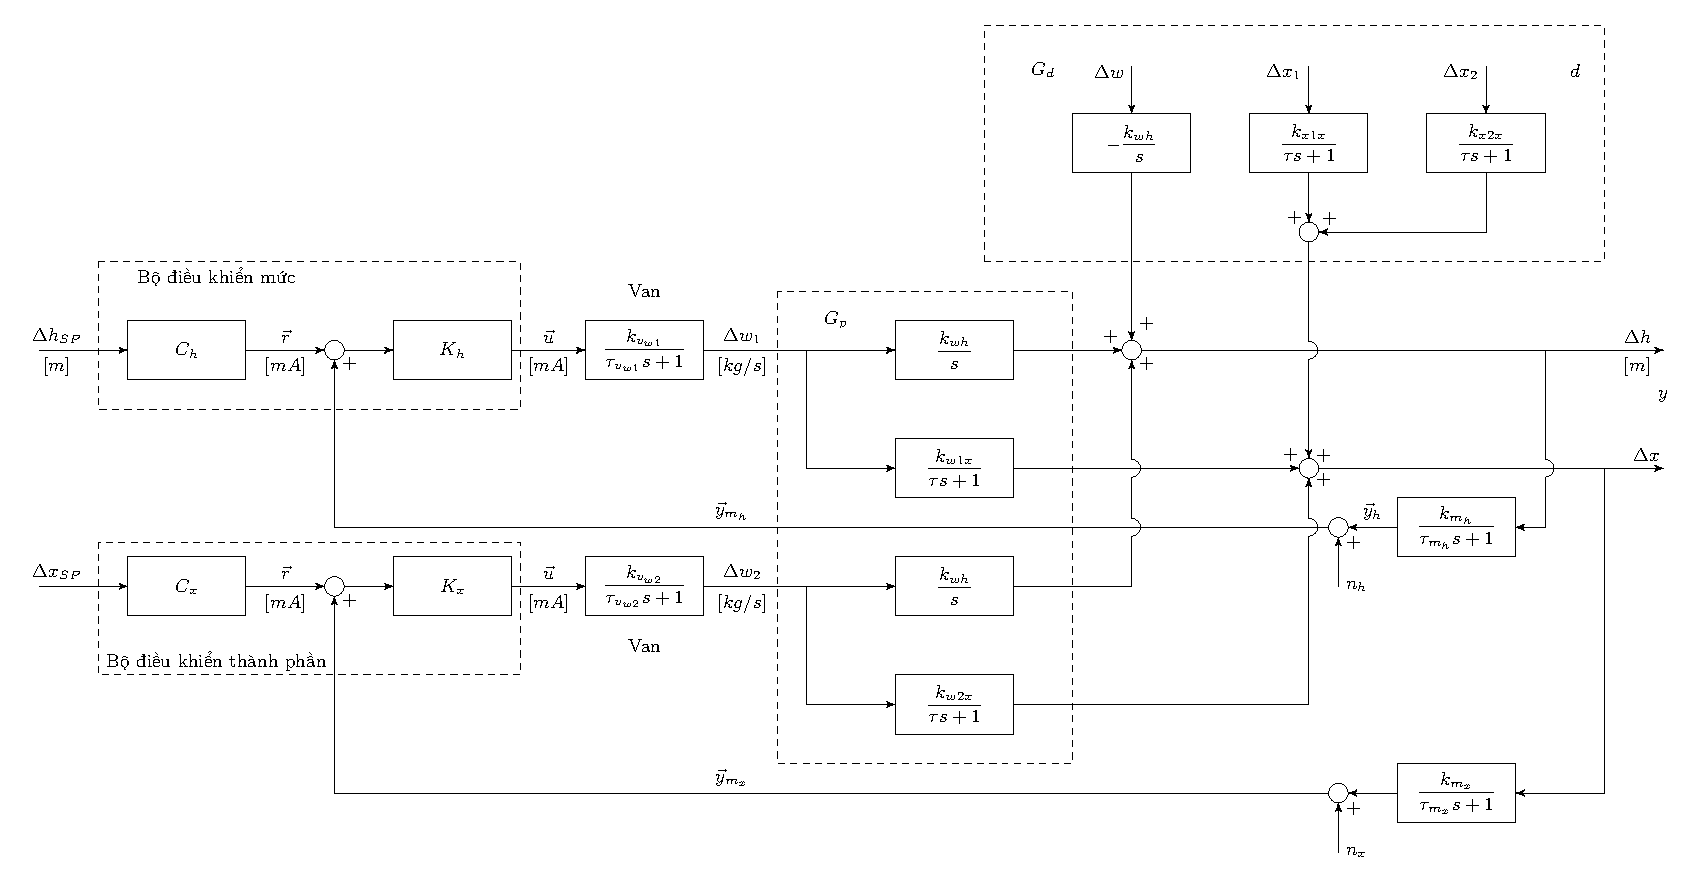
\includegraphics[scale=0.93]{section/mohinhhoalythuyet/images/binhchuachatlong-khuaytron-mohinh1-sodokhoi-cautrucdieukhienphanhoi}
    %                 }
    %         \end{center}
    %         \caption{Sơ đồ khối cho cấu trúc điều khiển phản hồi thiết bị khuấy trộn liên tục} \label{Fig:binhchuachatlong-khuaytron-sodokhoi-dieukhienphanhoi}
    %     \end{figure}
    % \end{landscape}
